%\clearpage
\section{Beamline Monitoring and Performance}
\label{performance}

%Several experimental runs have been completed using the CLAS12 detector with electron beams of up to $10.6$ GeV energy. 
During a typical experiment, Hall-B shift personnel monitor key beam parameters while beam delivery is controlled by operators in the 
Machine Control Center. The relevant beamline elements that are used to measure and monitor the key beam parameters are listed 
in Table~\ref{tab:elements}. 


\begin{table}[htp]
\caption{Elements of the Hall-B beamline actively monitored and controlled by the experiment shift personnel.}
\begin{center}
\begin{tabular}{|l|c|}
\hline
Name and description & Distance from center \\
&of the hall (meters) \\  \hline
Synchrotron Light Monitor& -43. \\ 
Wire harp 2C21 & -38.8 \\
nA-BPM 2C21A & -37.6  \\
M{\o}ller polarimeter & -31.5  \\
nA-BPM 2C24A & -24.5  \\
Wire harp 2C24 & -22.0  \\
Upstream halo monitors&-21.7 \\
Hall-B tagger dipole & -17.6  \\ \hline
Collimator & -15.3 \\
nA-BPM 2H01 & -8.0  \\ %\hline
Wire harp 2H01 & -7.4 \\
Midstream halo monitors& -3.9 \\ 
CLAS12 target & 0  \\ \hline
Downstream halo monitors & 7.5 \\
Beam viewer 2H04 & 24.0  \\
Dump, Faraday cup & 27.0  \\
\hline
\end{tabular}
\end{center}
\label{tab:elements}
\end{table}%

The Synchrotron Light Monitor (SLM) is a photomultiplier tube (PMT) that measures the synchrotron light 
generated in the last dipole magnet of 2C beamline that bends the beam into the Hall-B.  The amplitude of the SLM PMT signal is 
proportional to the beam current and is used to measure the helicity dependence of the beam charge. Due to its dependence on 
the beam position, it cannot be used as a long term beam current measurement device.


The nano-amp Beam Position Monitors (nA-BPMs) \cite{naBPM} measure the beam current and relative beam position in the transverse, 
or {\it x-y}, plane ($z$ is along the beam direction).  The beam position in each direction is measured to an absolute accuracy 
of 50 $\mu$m. The beam current can be measured to an accuracy of $\sim 1\%$ at beam currents above 10 nA, stable over weeks of
running.  Information from the nA-BPMs can also be used in a feedback  loop to keep the beam position fixed.

The wire harps \cite{wireharp} are used to measure the transverse beam profile. These are devices with 25-$\mu$m tungsten wires 
mounted in the horizontal and vertical directions on a support fork that moves the wires into the beam at $45^\circ$. As 
the harp moves into beam, count rates from beam halo counters are combined with the wire position information to determine the beam profile.
Since this is an invasive measurement, it is performed primarily during beam setup or when other devices indicate a problem with the beam. 

The beam halo counters are PMT-based devices located at various positions along the beamline and are mounted very close to the 
beam; usually strapped directly to the beam pipe. The PMTs have either scintillating or Cherenkov-light-producing plastic mounted on 
the photocathode. In addition to providing count rates for the wire harps, these counters are sensitive to any beam halo or undesirable 
beam interactions. These counters are the main tools to monitor beam-induced background in the hall and, along with the BOM, provide 
feedback signals for the machine fast shutdown system (FSD). The FSD will stop beam delivery in the case of excessively high background
rates in order to protect the detectors. 

Other devices that Hall B uses to monitor and measure beam parameters are the M{\o}ller polarimeter located in the upstream tunnel for beam 
longitudinal polarization measurement, a Faraday cup in the downstream tunnel (electron beam dump) for precise beam current measurement, 
and a beam viewer that looks at a retractable fluorescent screen installed before the Faraday cup for visual verification of beam transport to 
the dump.     

The Experimental Physics and Industrial Control System (EPICS) \cite{EPICS} is used for monitoring the beam delivery and for control 
of the beamline devices. Graphical User Interfaces (GUIs) for each application are built using the CS-Studio tools \cite{CS-Studio}. All 
variables available in EPICS are archived using the Jefferson Lab MYA data archiver \cite{MYA}. For continuous monitoring of the beam
and the state of the beamline devices, one single GUI was deployed that contains monitored quantities from the beam halo counter rates,
magnets, vacuum, cryotarget, beam positions and currents, as well as state of moving devices. For convenience of monitoring, a timeline 
of counter rates, along with BPM positions and beam current readings can be displayed separately.  

%\begin{figure*}[t]
%\begin{center}
%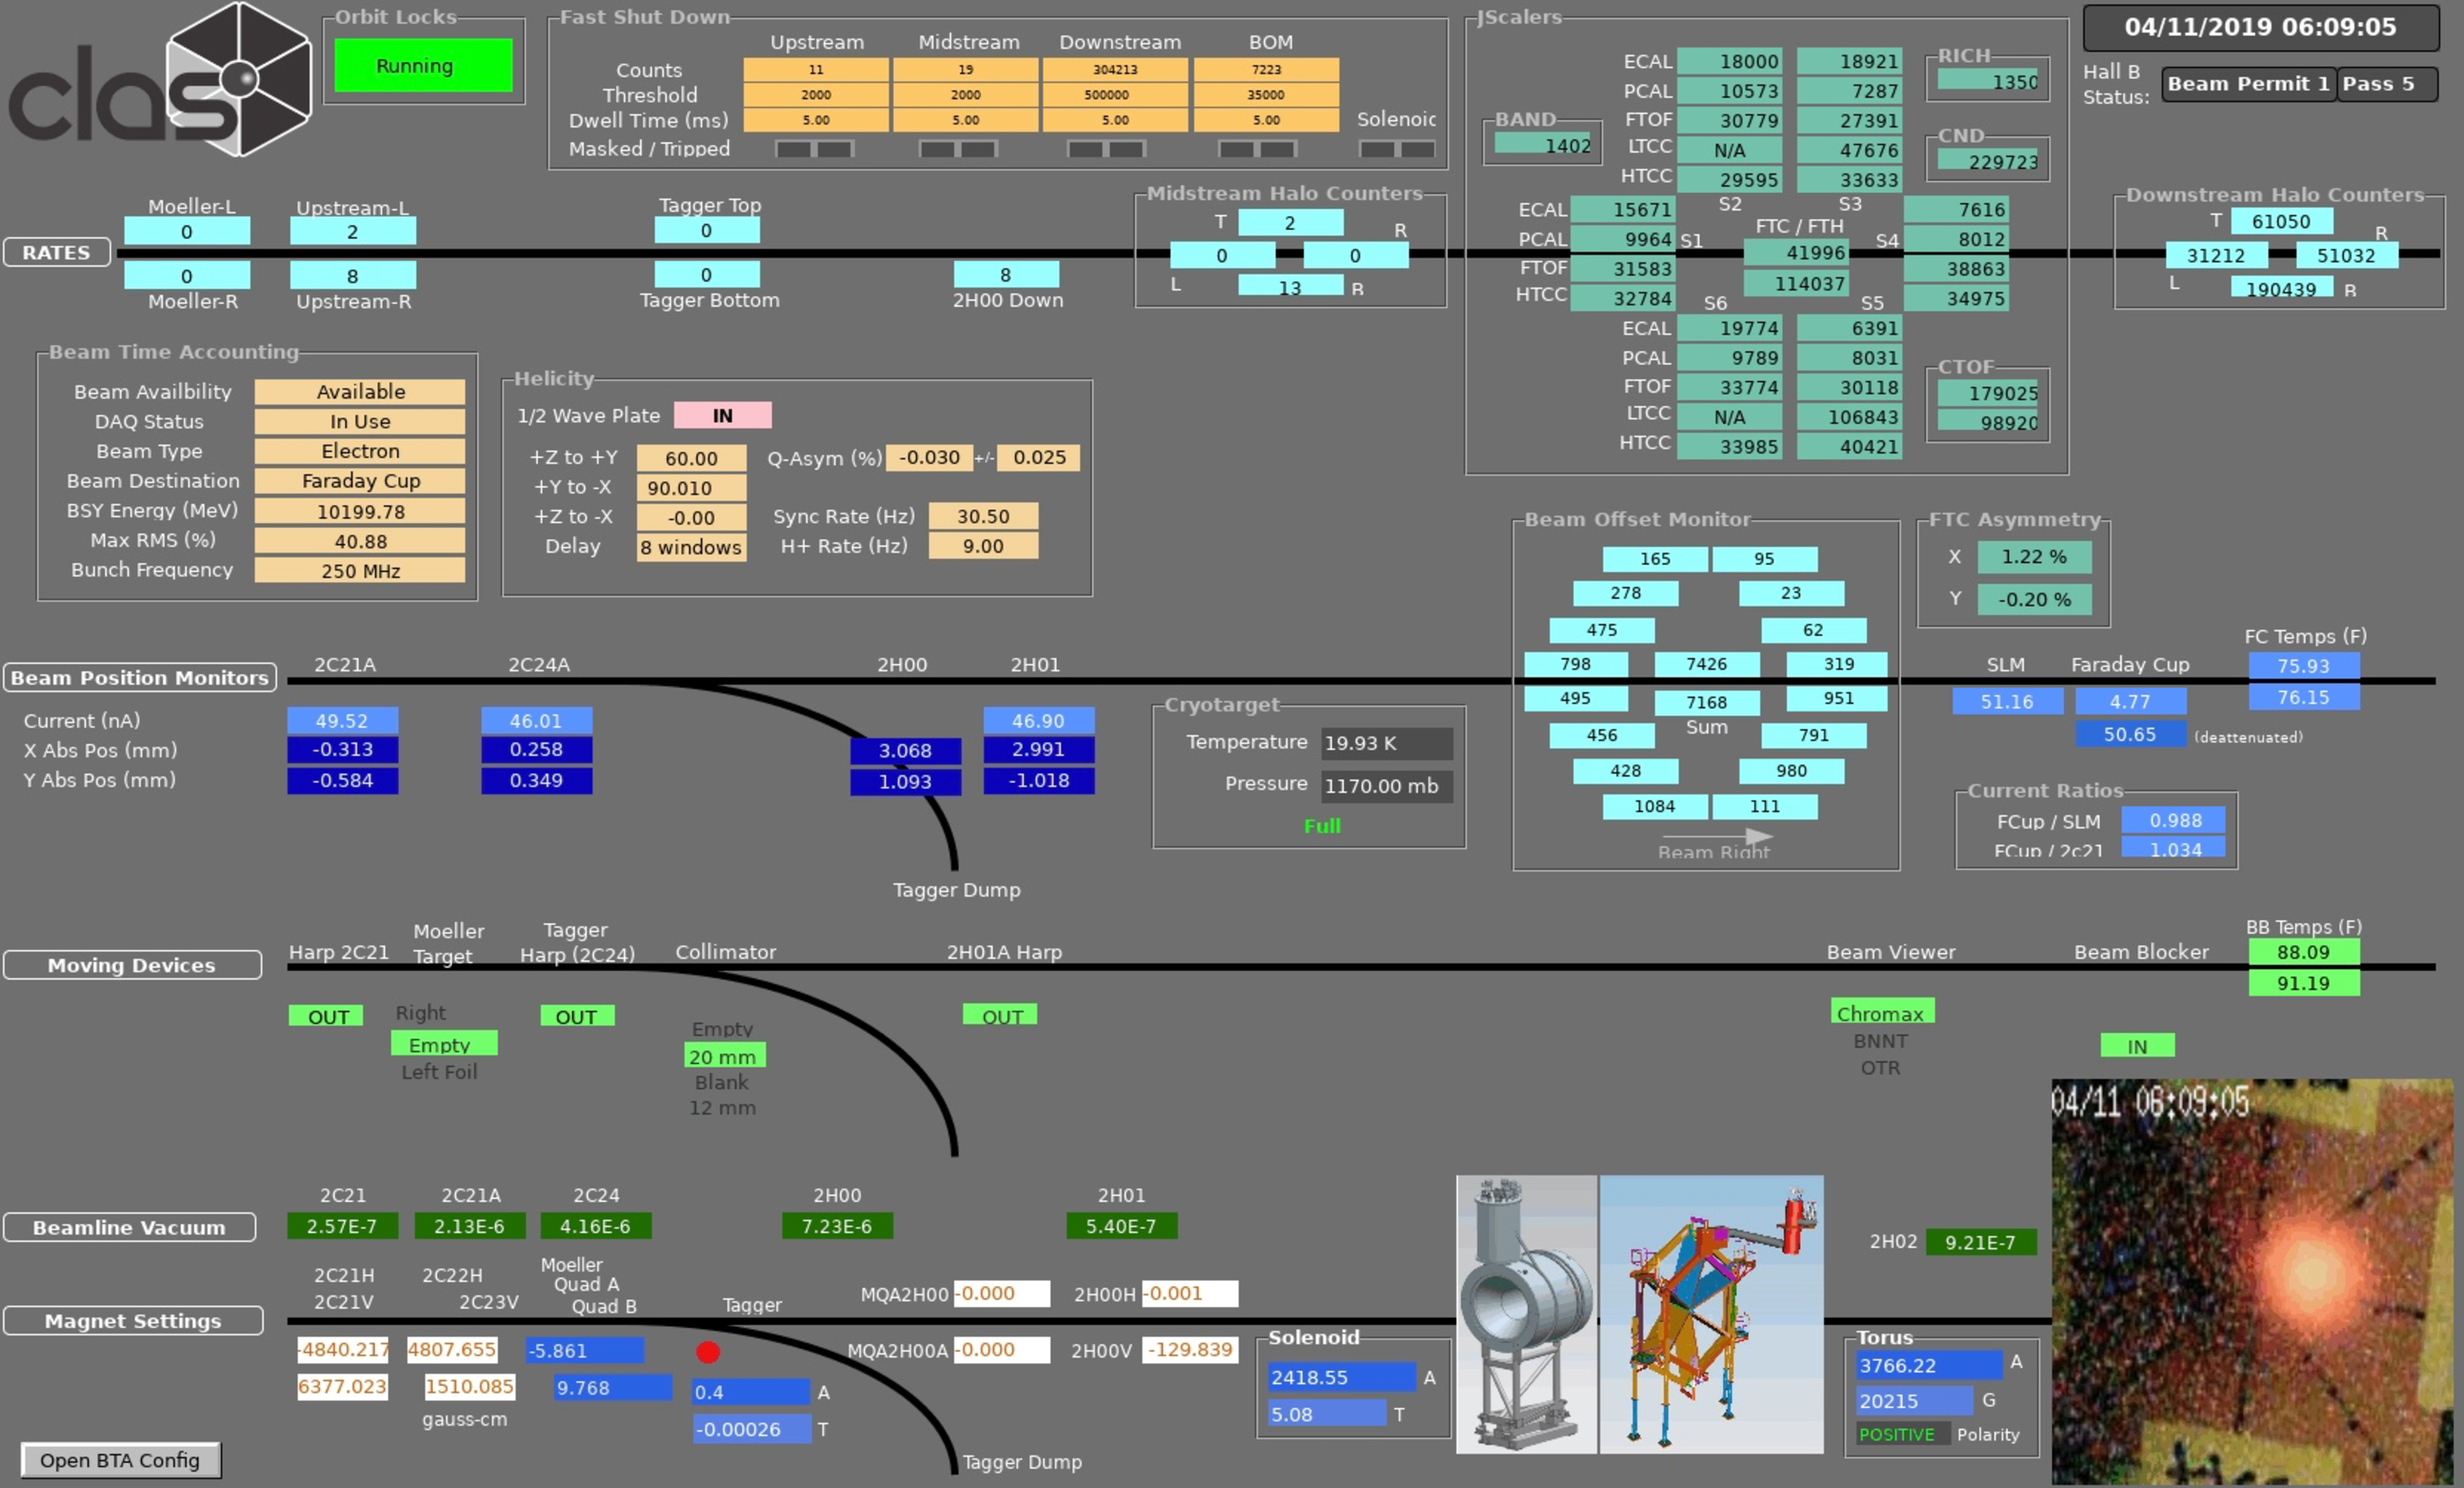
\includegraphics[width=0.95\textwidth]{main_gui.pdf}
%	\caption{The main Graphical User Interface (GUI) for monitoring of beamline devices, detector rates, and magnets.}
%\label{fig:mgui}
%\end{center}
%\end{figure*}



Establishing a production quality electron beam for experiments in Hall B is a two-step process. First, the beam is delivered and tuned in 
the 2C beamline in the Hall-B upstream tunnel. During this tuning process the beam is dumped on the tagger yoke to protect CLAS12 
detectors from excessive radiation exposure. Once the 2C beamline is tuned, the beam is then sent to the downstream electron dump and 
tuned onto the CLAS12 target. During the tuning process, the beam profile and transverse position are optimized using the information from 
the wire harps, the nA-BPMs, and the beam halo counters.  The beam is accepted for physics production running when all the relevant 
parameters are within expected limits. After production beam has been established,  limits on the halo counter rates, beam position, and 
beam current are set in the CS-Studio alarm system to help Hall-B shift personnel to monitor the beam quality when running experiments.  


%\subsection{Establishing beam for physics}



%\subsection{Beam alignment}


\subsection{Beam profile and position stability}

Establishing and maintaining a high-quality beam is important for obtaining high-quality physics data. Once the beam has been established, 
scans using the wire harps and nA-BPMs are stored in the MYA archive and are used as reference values over the course of an experimental
running period. Figure~\ref{fig:profile}  shows the {\it x--} and {\it y--}profiles measured with wire harps 2C21 and 2H01, located in the upstream 
tunnel of Hall B and at 7.4 m upstream of the target, respectively. During these measurements, the beam was delivered to the Faraday cup.
Figure~\ref{fig:prof2h01} shows a histogram of the {\it x-} and {\it y-}widths for sixteen 2H01 harp scans taken over a two month running
period.  The beam width in both directions fluctuates between $180~\mu$m to $300~\mu$m with an average value of $250~\mu$m. 

\begin{figure}[ht]
\begin{center}
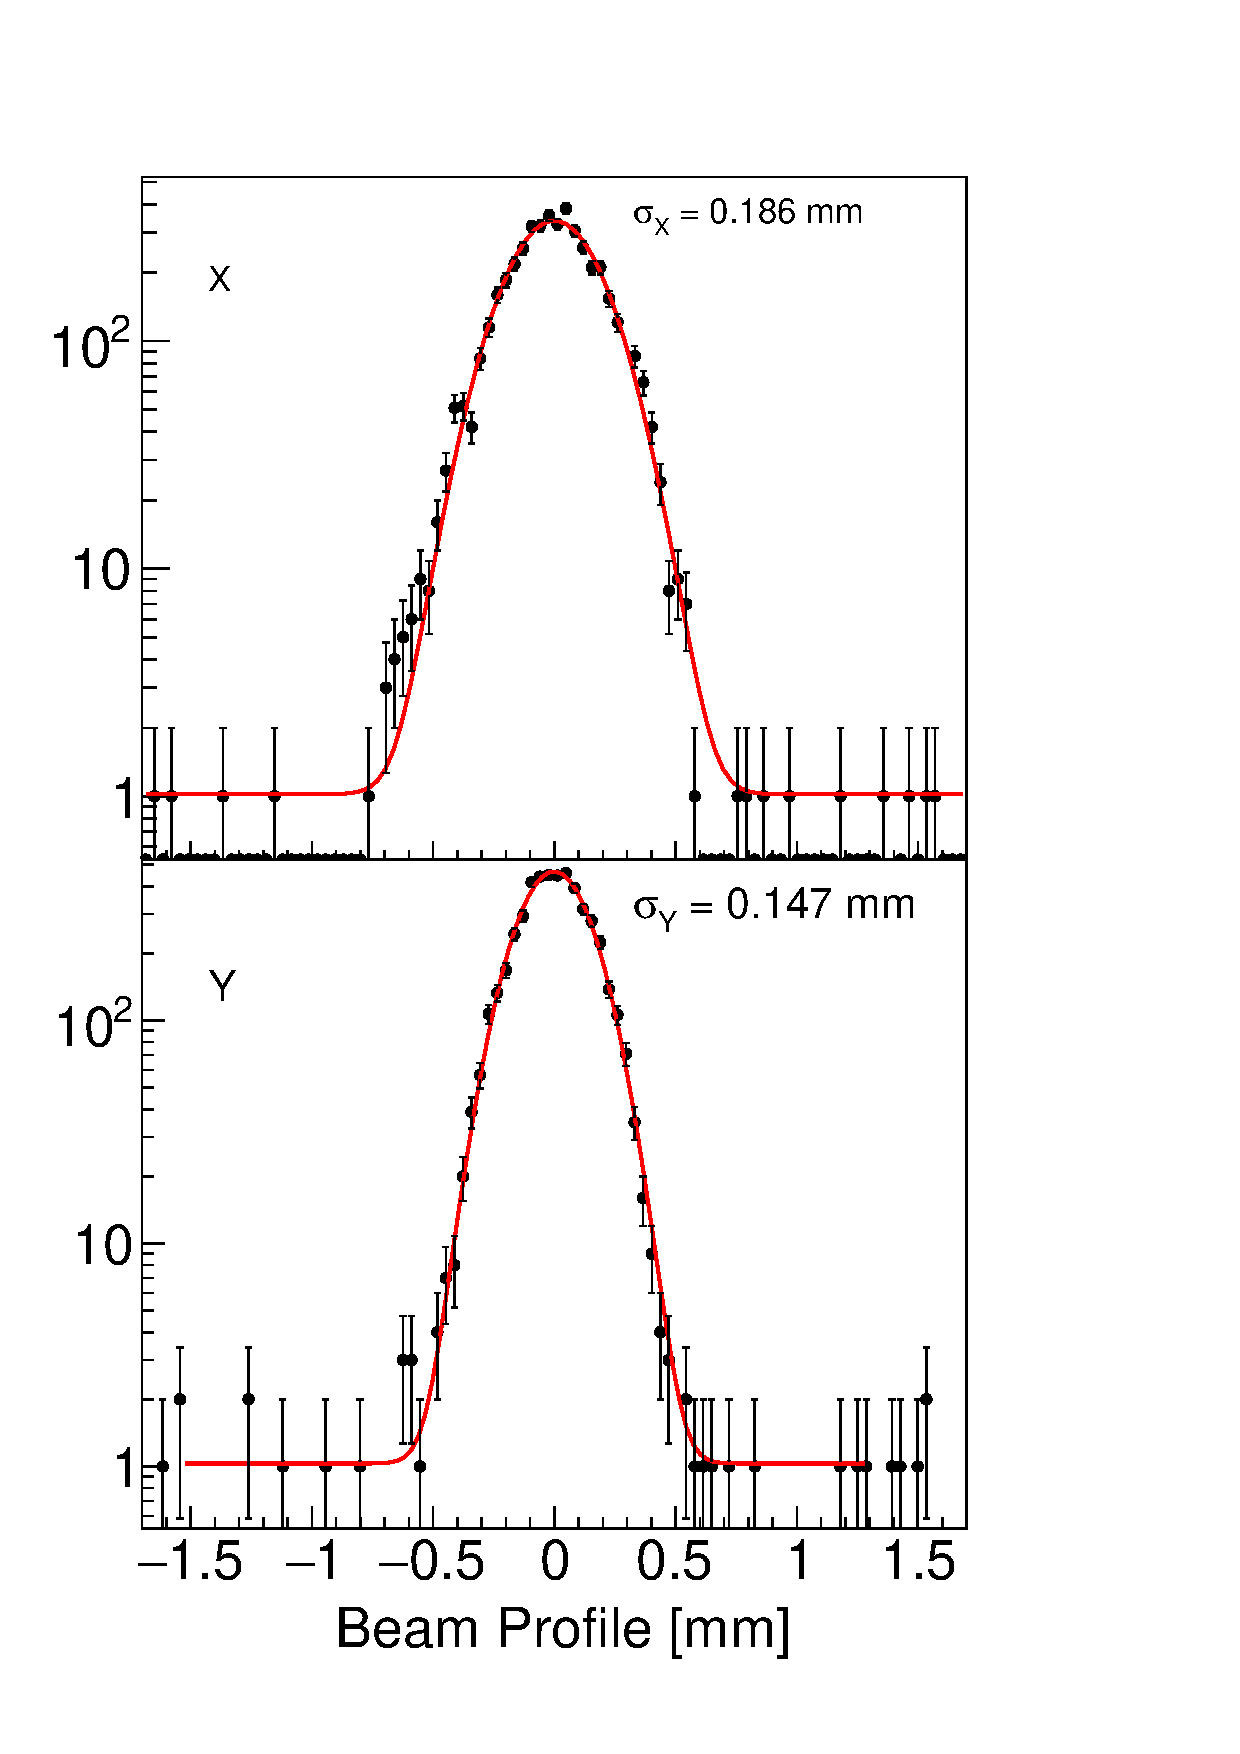
\includegraphics[width=0.23\textwidth]{2C21_fits.pdf}
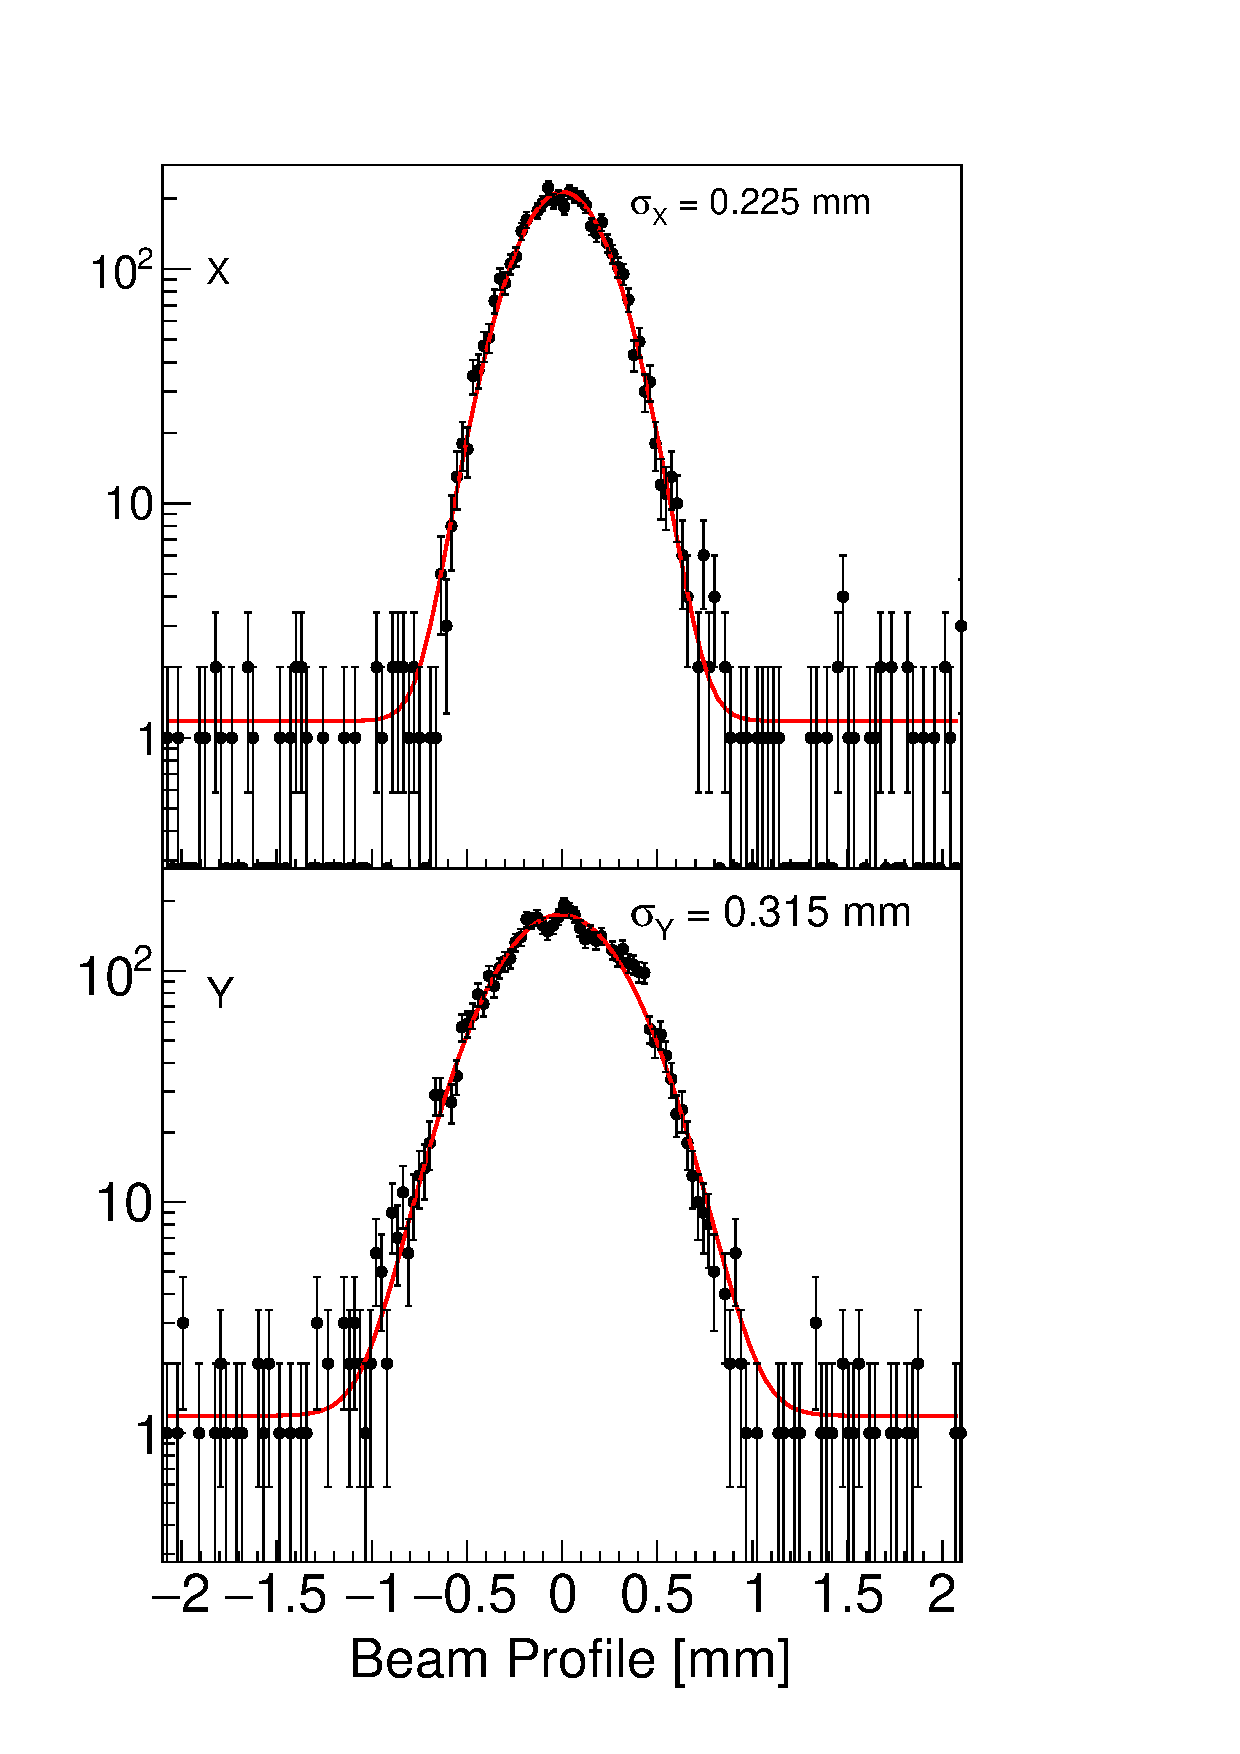
\includegraphics[width=0.23\textwidth]{2H01_fits.pdf}
%\includegraphics[width=0.225\textwidth]{tgr_fits.pdf}
	\caption{Beam {\it x--} (top) and {\it y--}profiles (bottom) measured using the wire harp scanners at 2C21 (left) and at 2H01 (right). The red
	curve is a Gaussian fit with the width shown by the $\sigma$ values. }
\label{fig:profile}
\end{center}
\end{figure}

\begin{figure}[ht]
\begin{center}
%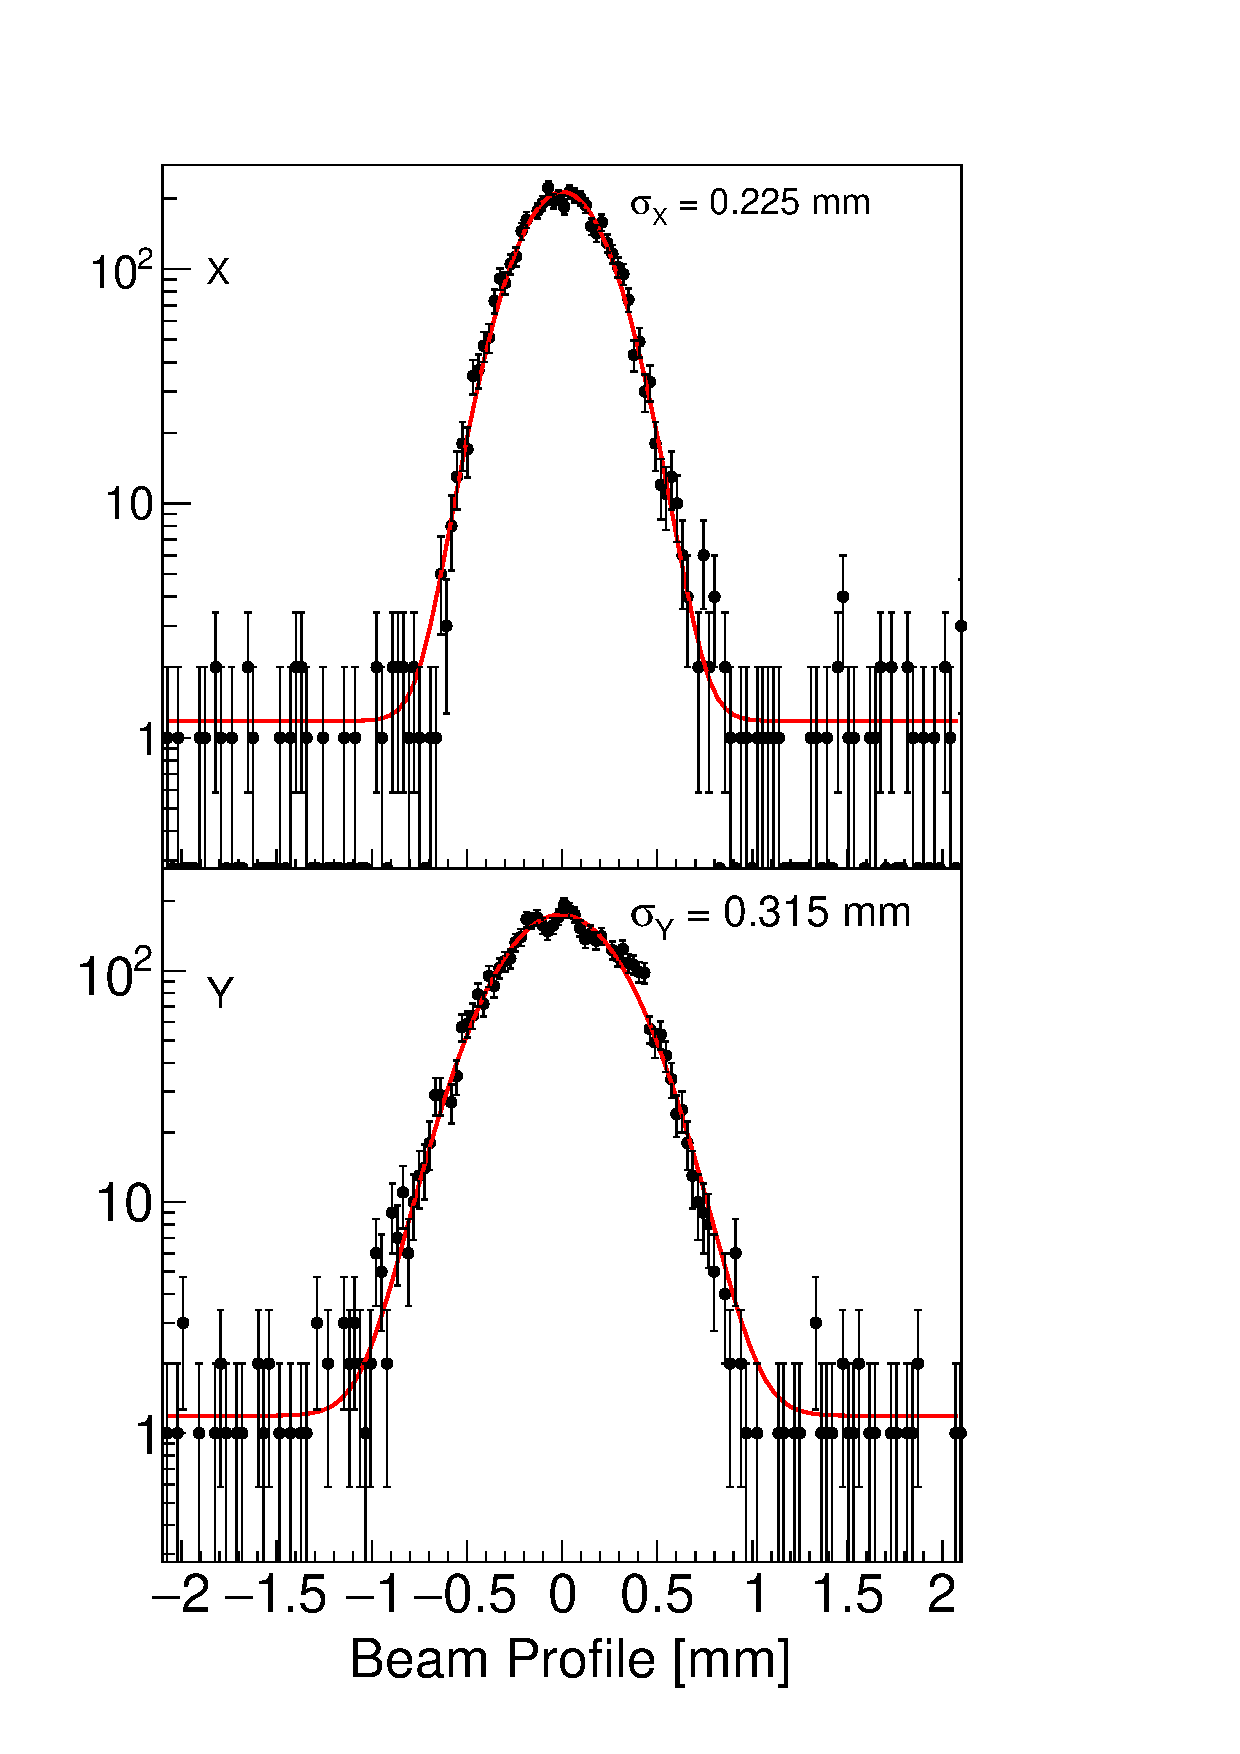
\includegraphics[width=0.225\textwidth]{2H01_fits.pdf}
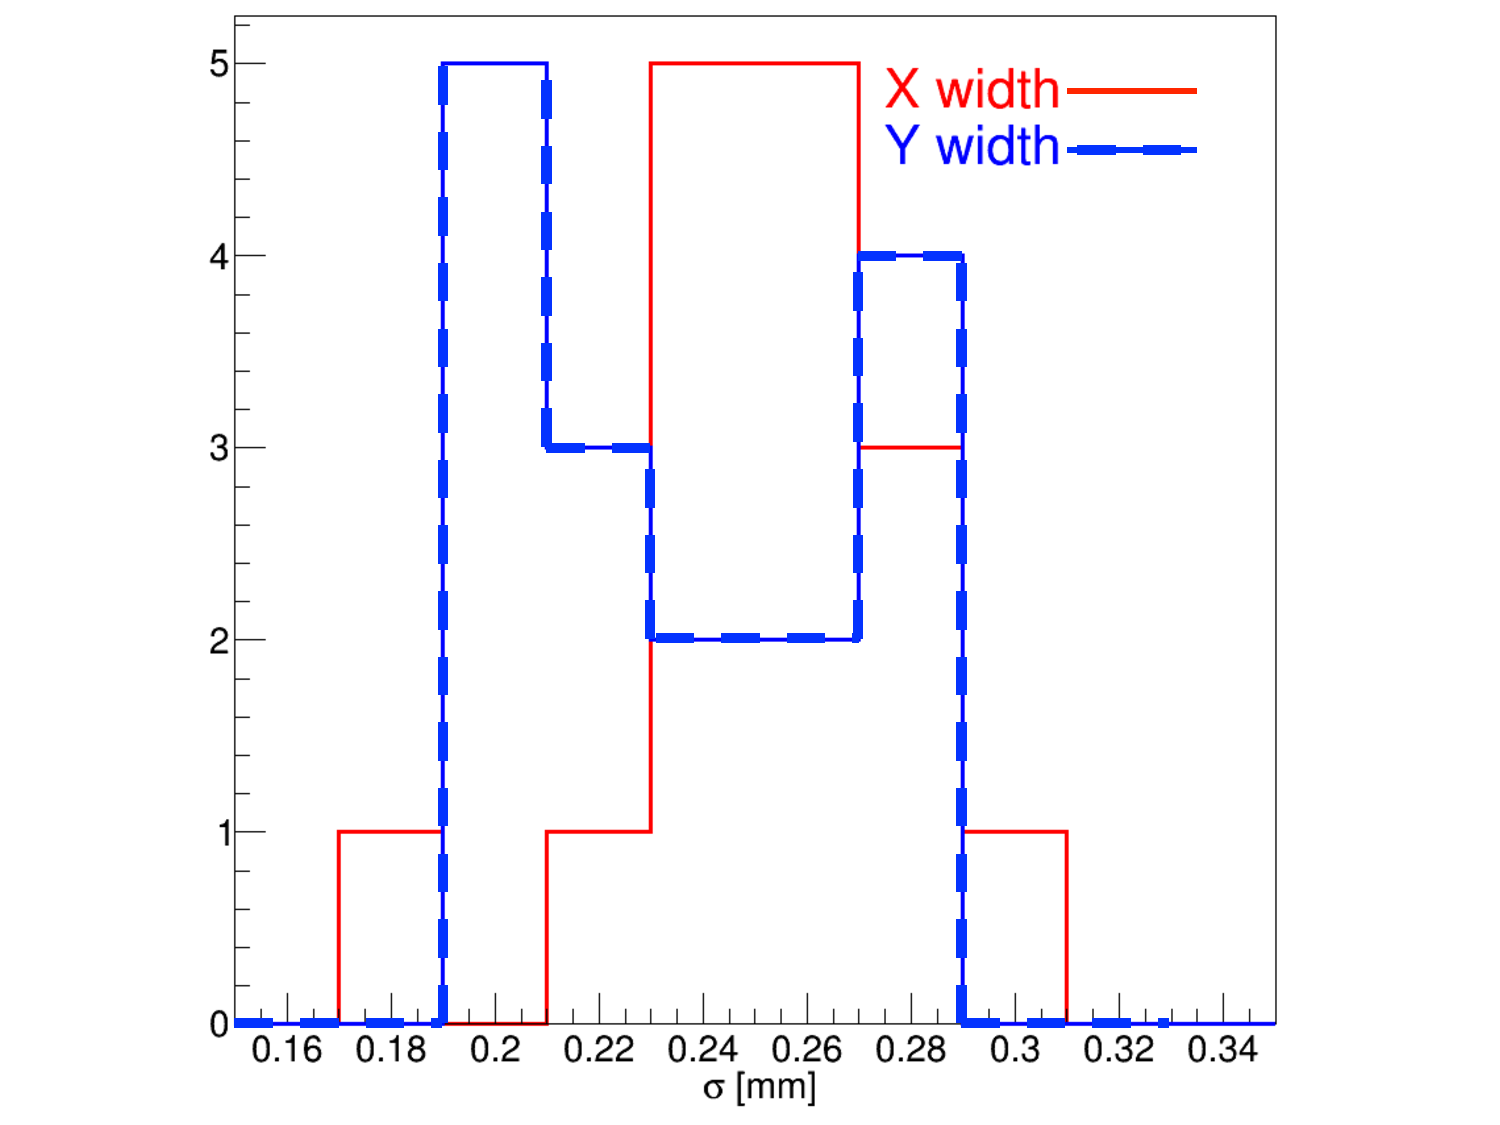
\includegraphics[width=0.4\textwidth]{BeamWidth.pdf}
	\caption{Beam width measured with the 2H01 wire harp over two months of running. The {\it x--}width is shown in solid red and the 
	{\it y--}width is shown in dashed blue.}
\label{fig:prof2h01}
\end{center}
\end{figure}

After the beam has been established for physics running, its position and current stability are continuously monitored using the halo 
counter rates and the nA-BPMs. Figure~\ref{fig:position} shows the the distribution of the {\it x--} and {\it y--}positions about the mean at the 
2H01 nA-BPM. The RMS of both distributions is on order of $20~\mu$m. Such stability is largely due to use of the beam orbit lock system 
that uses the position readings of nA-BPMs to drive horizontal and vertical correctors that keep the position of the beam at the set points 
established at the start of a running period.

\begin{figure}[ht]
\begin{center}
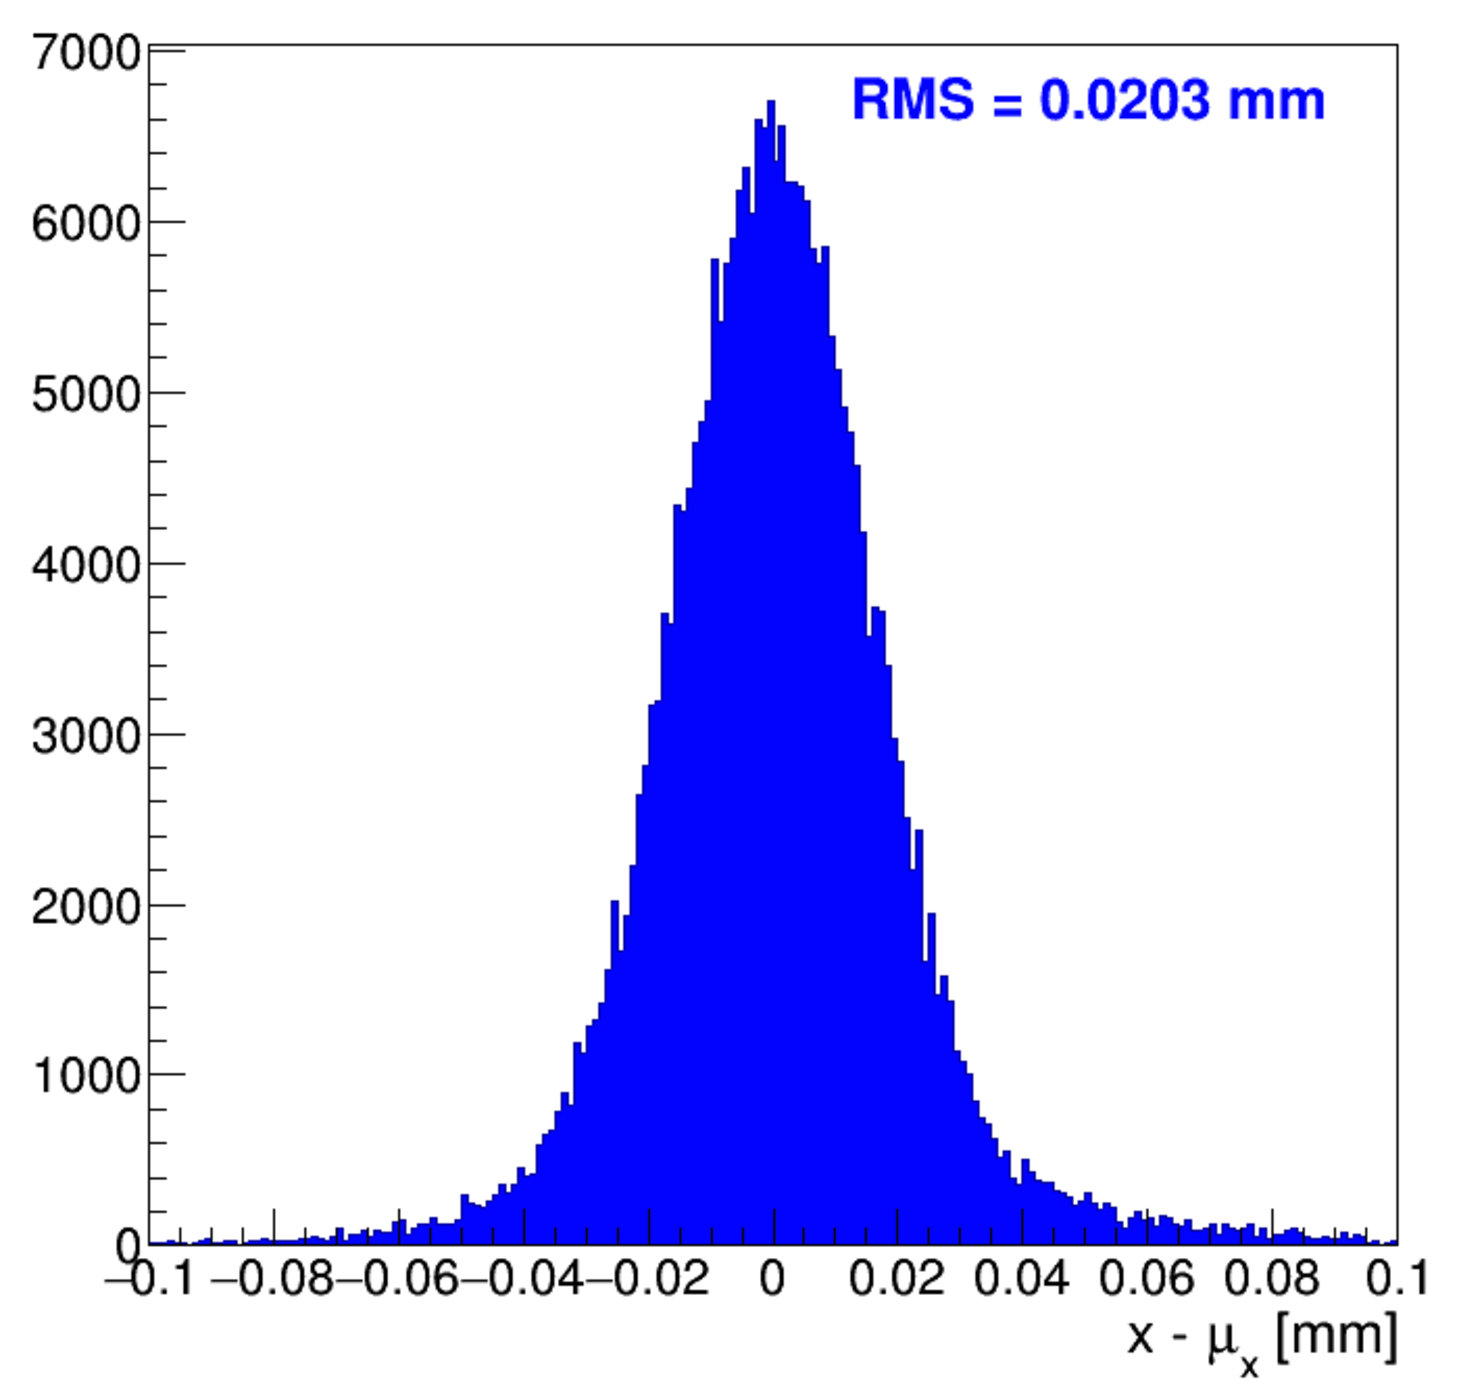
\includegraphics[width=0.234\textwidth]{position_2h01x.pdf}
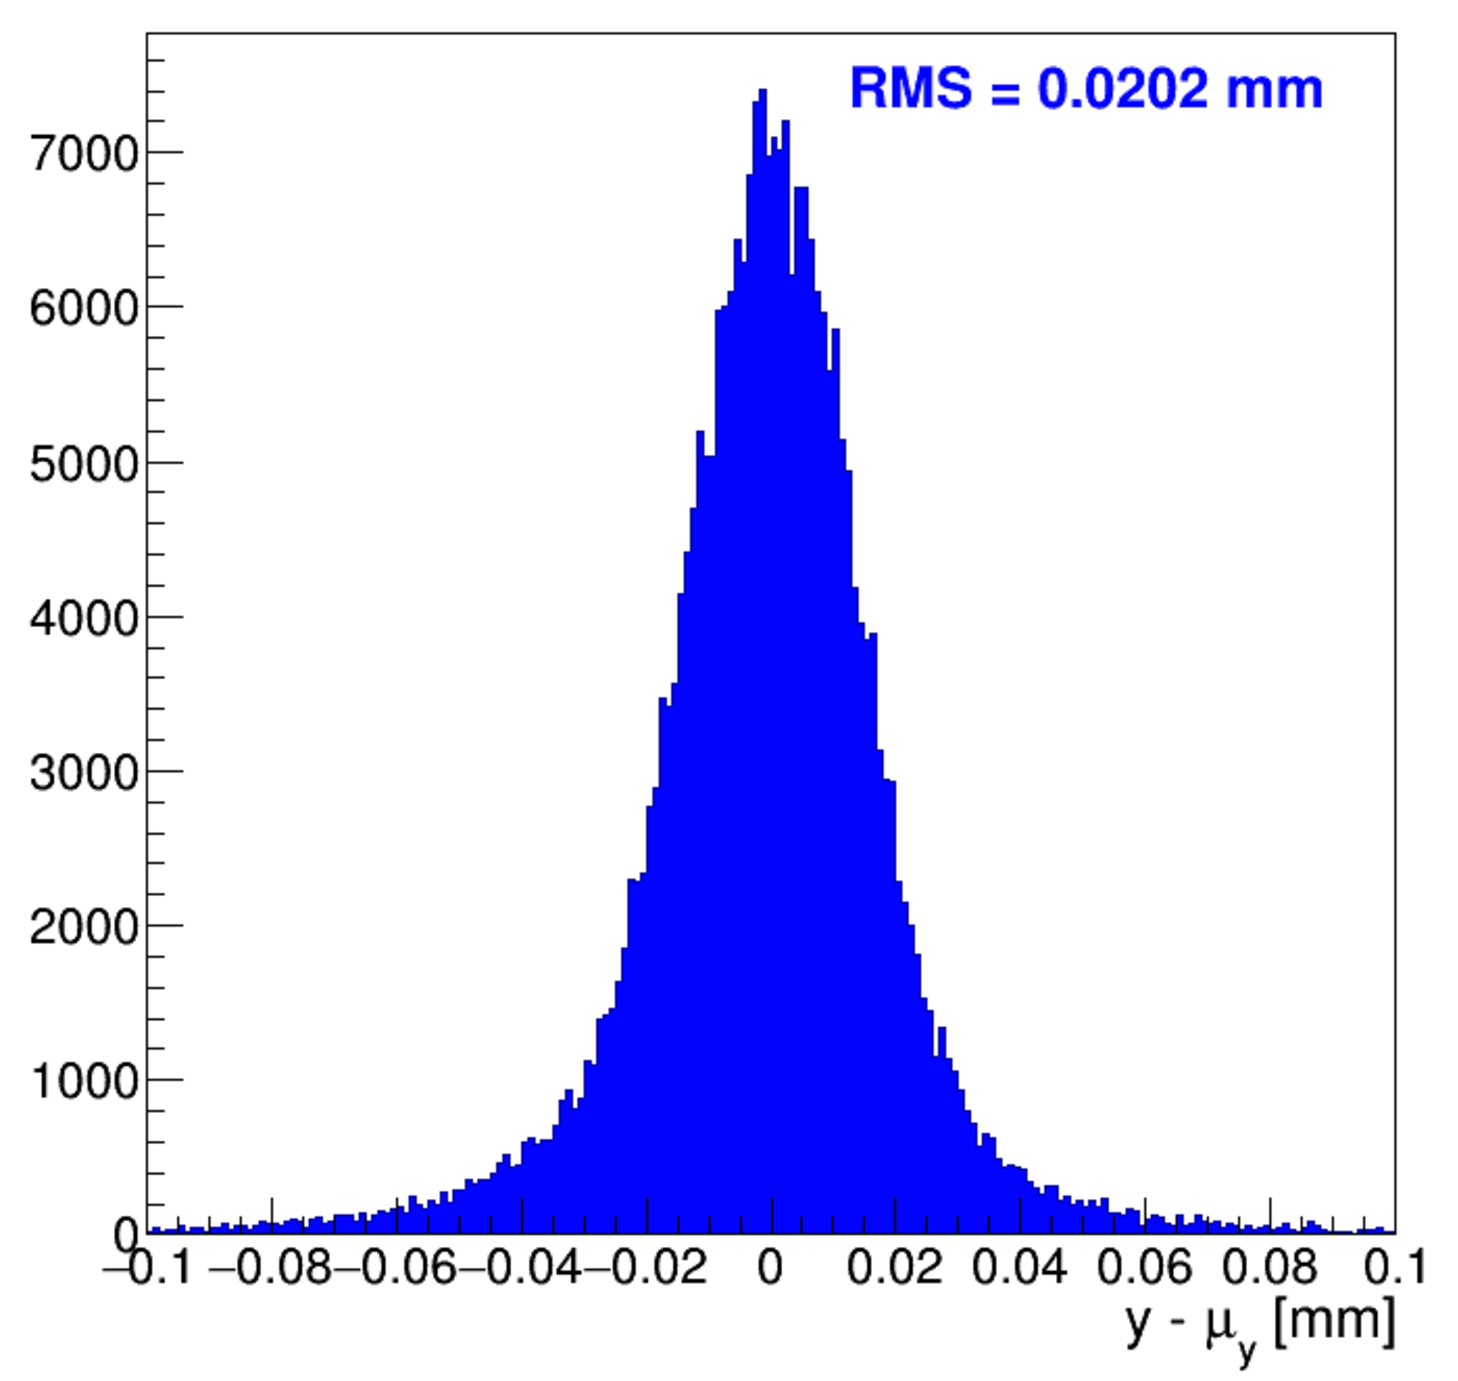
\includegraphics[width=0.234\textwidth]{position_2h01y.pdf}
\caption{Beam position deviations, $x-\mu_x$ (left)  and $y-\mu_y$ (right), over a month of running as measured by the 2H01 nA-BPM. }
\label{fig:position}
\end{center}
\end{figure}



%\subsubsection{Feedback Test of the FSD system}


%The CEBAF Fast Shut Down (FSD) system provides permissive signals to the injector gun. 
%If the permissive is removed, the gun shuts 
%off within 20 $\mu$s. 
%One of inputs to the FSD system was the sum of the HPS halo counter rates. 

%The output signal of a logic module that was {\it OR} of four halo counters installed downstream of the SVT protection collimator was sent to a custom FSD module. The module initiates a FSD signal if the rate on the input exceedes the set threshold within defined time window.

  

%%%%%%%%%%%%%%%%%%%%%%%%%%%%%%%%%%%%%%%%%%%%% F I G U R E %%%%%%%%%%%%%%%%%%%%%%%%%%%%%%%%%%%%%%%%%%

%%%%%%%%%%%%%%%%%%%%%%%%%%%%%%%%%%%%%%%%%%%%% F I G U R E %%%%%%%%%%%%%%%%%%%%%%%%%%%%%%%%%%%%%%%%%%


%\subsection{Beam halo}

\subsection{Beam charge measurement}
\label{sec:FC}

An accurate measurement of the total amount of beam charge incident on the target during an experiment is vital for the measurement of 
experimental cross sections. The Hall-B Faraday cup (FC) is the main tool to obtain an accurate {\it absolute}  beam current  
measurement. A description of the Faraday cup and its readout electronics can be found in Ref.~\cite{CLAS}. 
Since the Faraday cup does not have active cooling, it is limited to 175 W of beam power for long exposures. 
However, most of the CLAS12 experiments will run with beam currents that exceed the power limit of the FC, thus requiring another method
of measuring the beam current. The other devices used to monitor the beam current during the experiment are the nA-BPMs and the SLM, 
but these devices do not have the long-term stability to provide the accuracy needed over the weeks-long course of an 
experiment.\footnote{The calibration of the nA-BPMs relative to the FC remains stable within a few \% for a period of time sufficient 
for coarse monitoring of the beam current during the experiment.}   

Instead, a 5-kW beam dump can be inserted in front of the FC during high-power running. This insertable dump, or beam blocker, is a 
water-cooled, 28-cm-long copper cylinder (19.5 radiation lengths).   While most of the beam is deposited in this beam blocker, the FC 
still measures a leak-through current that is proportional to the total beam current with a very high accuracy of better than 0.5\%. 
In order to use the FC current measurement with the blocker in, a beam-current attenuation factor, $A$, must be determined for every 
beam energy, so that the beam current is given by $I=A I_{FC}^{in}$, where $I_{FC}^{in}$ is the beam current measured at the FC when the
beam blocker is in. 

To calibrate the attenuation factor, first, a scan of the beam current up to the highest current required by the experiment is done 
without the beam blocker. The scan is quick so as to not overheat the FC.  These data are used to calibrate the nA-BPM current readings 
relative to the FC with a calibration factor given by $C={I_{BPM}}/{I_{FC}},$
where $I_{BPM}$ and $I_{FC}$ are the currents measured by the nA-BPM and FC, respectively. The left panel of Fig.~\ref{fig:2c21fc} 
shows a distribution of $C$ for a range of beam currents from 15 to 80 nA at a beam energy of 10.67 GeV using the 2C21 nA-BPM.
The distribution has a mean of $\langle C\rangle=1.057$ and Gaussian width of $\sigma_C=0.0038$, which we use to determine 
the relative uncertainty in the calibration factor of $\delta C/C=\sigma_C/\langle C\rangle=0.36$\%.
 
\begin{figure}[ht]
\begin{center}
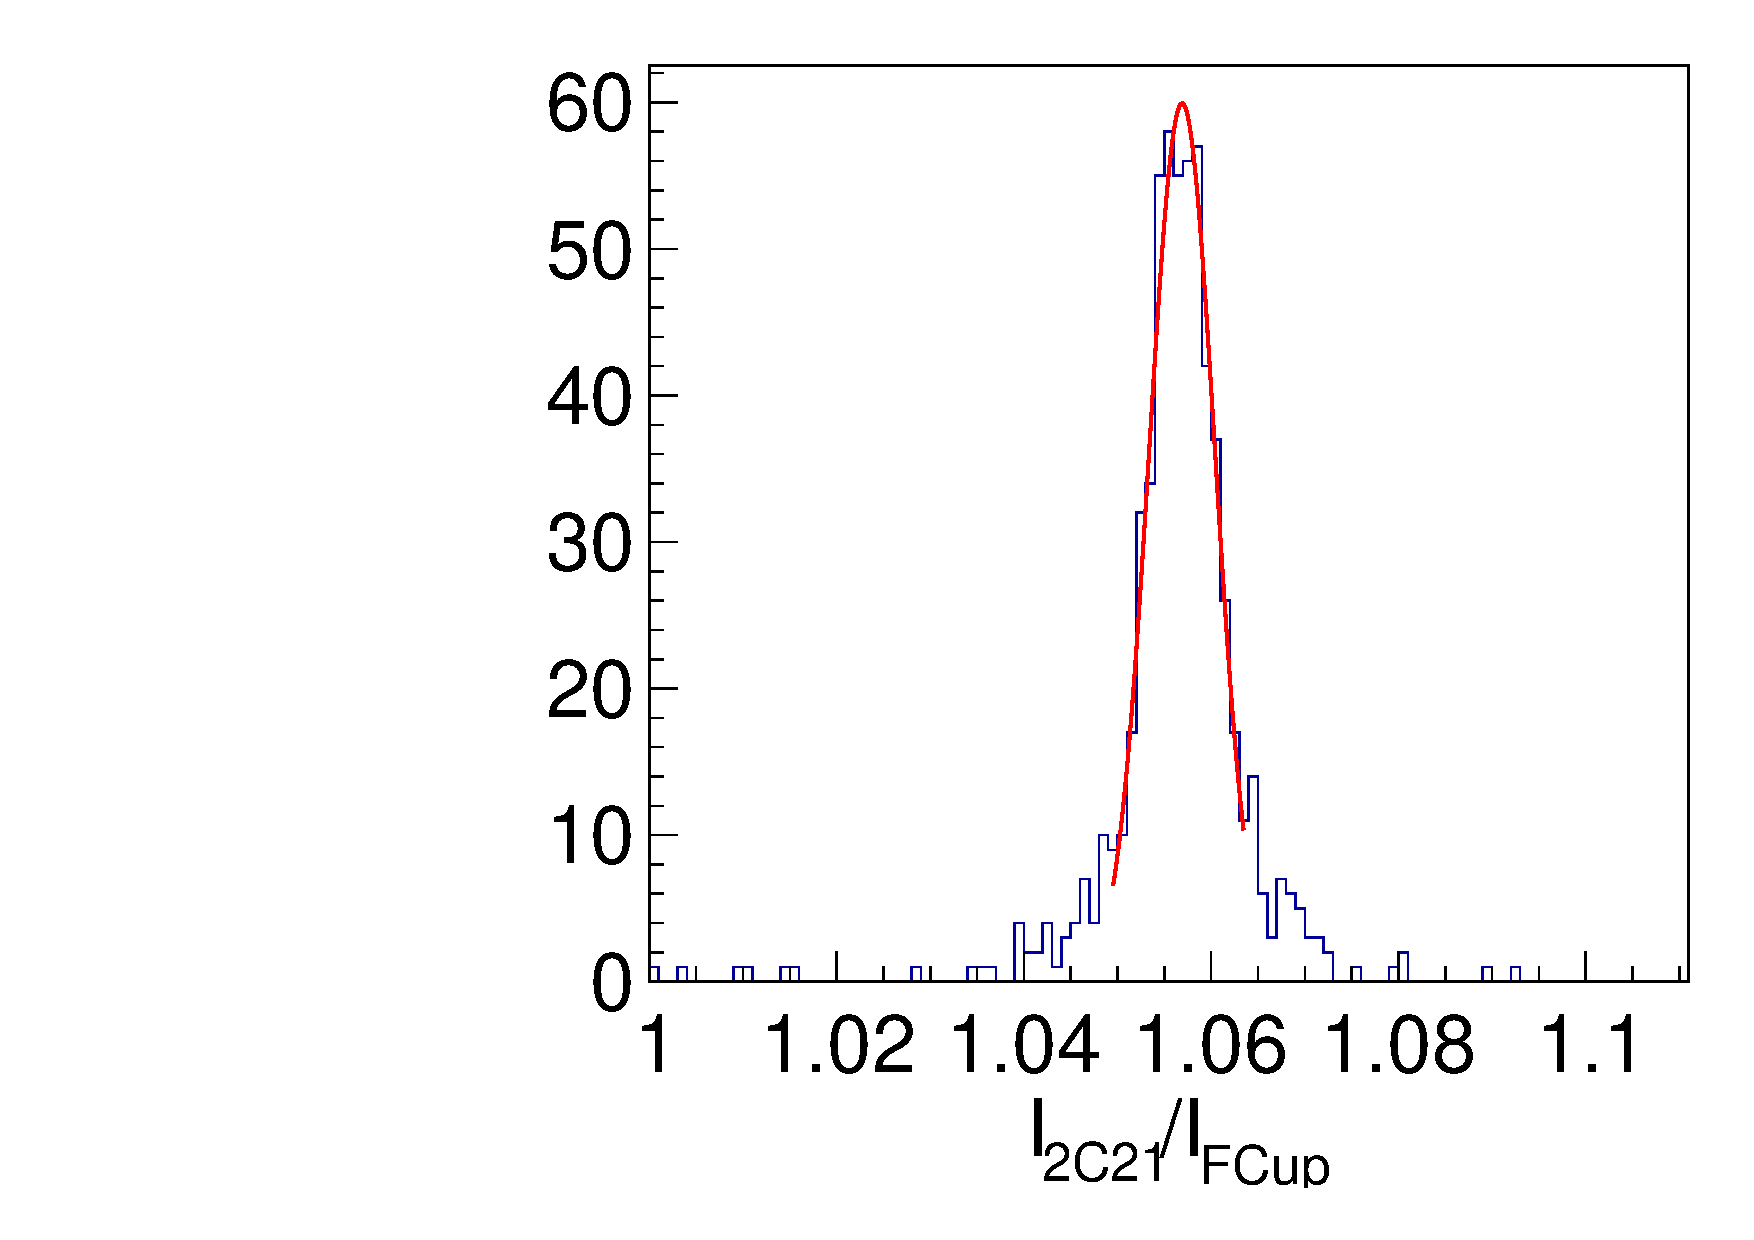
\includegraphics[width=0.23\textwidth]{fCup_2C21_ratio_highcurr.pdf}
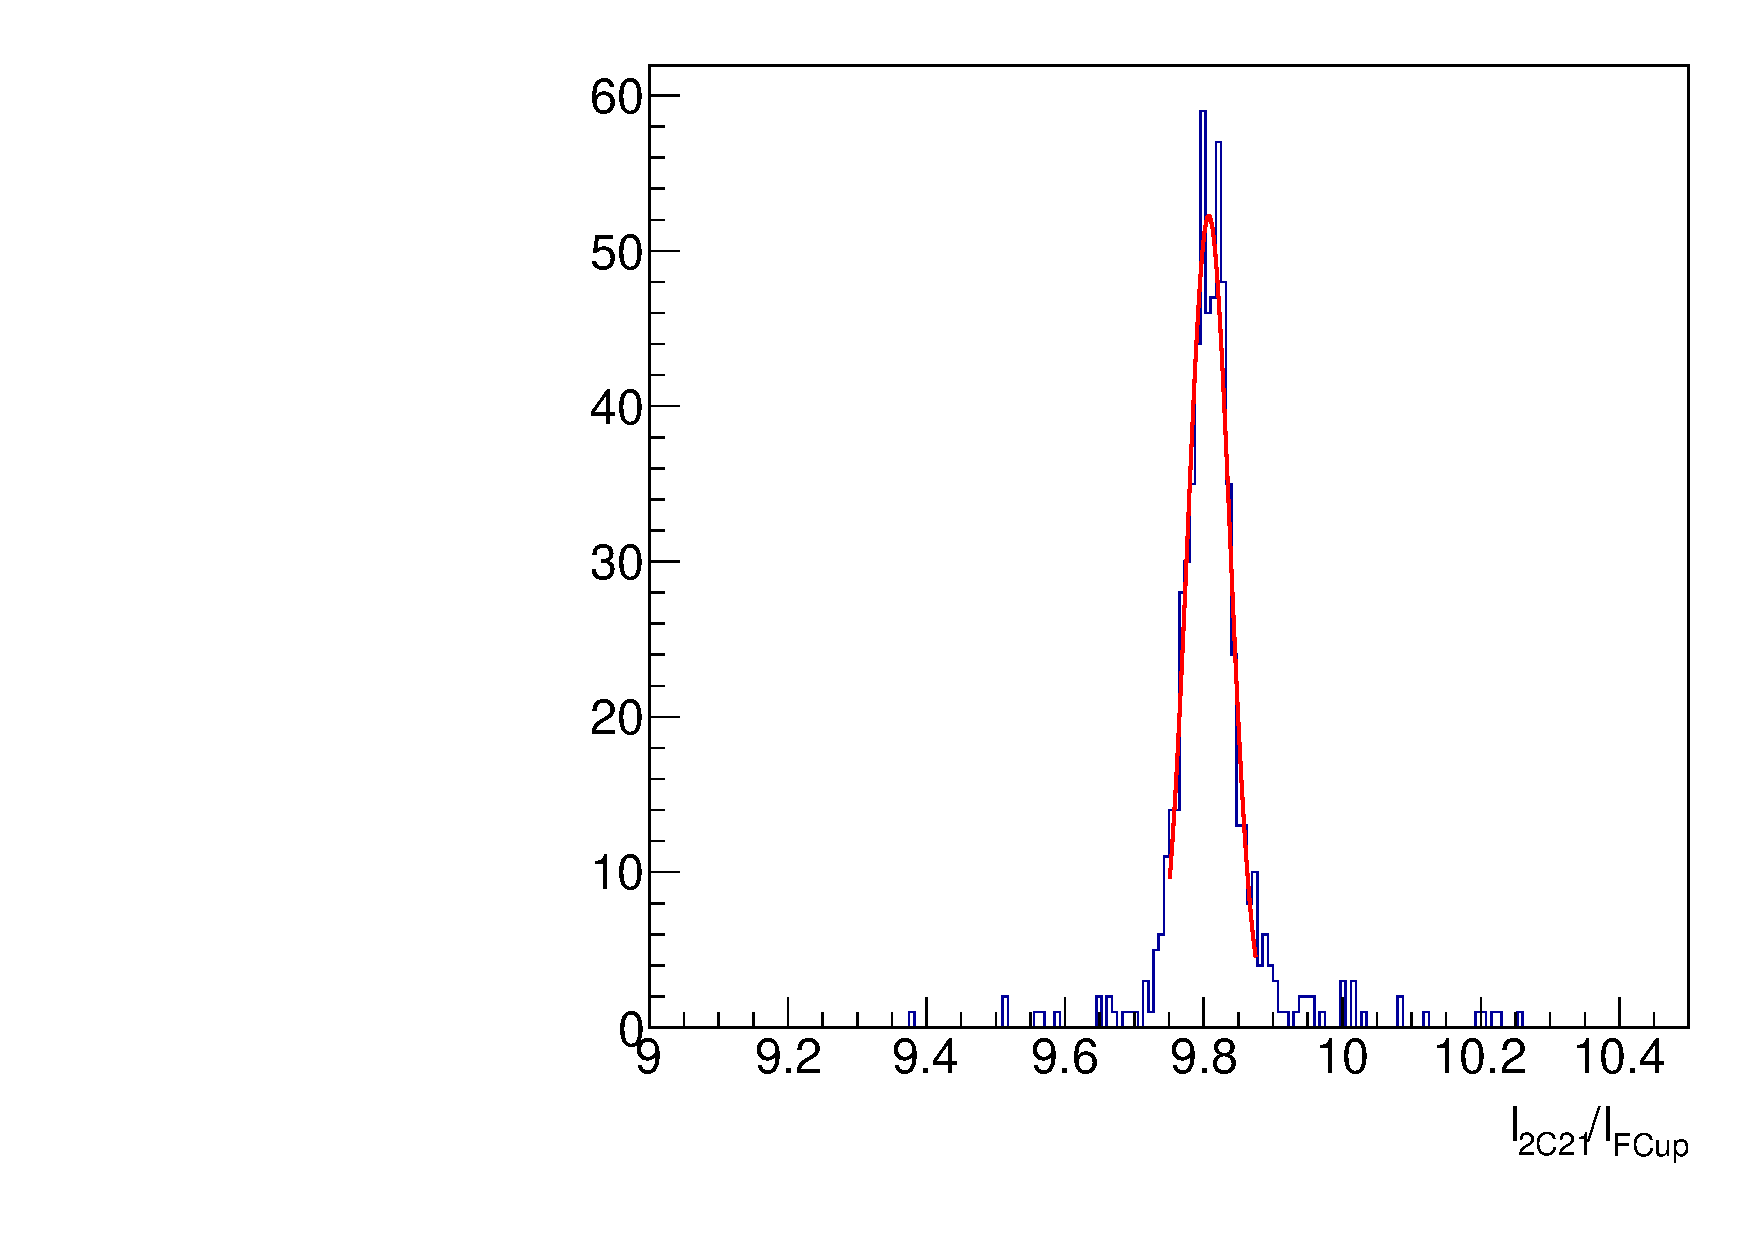
\includegraphics[width=0.23\textwidth]{BB_attenuation_2c21_highcurr.pdf}
\caption{The ratio of beam currents measured by the 2C21 nA-BPM and the Faraday cup without (left) and with (right)  the insertable beam
 blocker. Each distribution has been fit with a Gaussian to obtain the means and widths given in the text.}
\label{fig:2c21fc}
\end{center}
\end{figure}

 
In the second step, a similar current scan is performed but with the insertable beam blocker in place. Using the now
calibrated values of the nA-BPM current reading from the first step, the attenuation factor is given by 
$A=I_{BPM}^{in}/{I_{FC}^{in}}$.
The distribution of $A$ is shown in the right panel of Fig.~\ref{fig:2c21fc}, which has also been  obtained for a range of beam 
currents from 15 to 80 nA at a beam energy of 10.67 GeV using the 2C21 nA-BPM.  The distribution has a mean of $\langle A\rangle=9.807$
and a  Gaussian width of $\sigma_A=0.0306$, which leads to a relative uncertainty of $\delta A/A=\sigma_A/\langle A\rangle=0.31$\%. 
Combining the uncertainties from the calibration of the nA-BPMs and the attenuation factor leads to a total relative uncertainty in the 
blocker-in FC current measurement of $\delta I_{FC}/I=0.48$\%. 

A simultaneous measurement of the attenuation factor has been done using the 2C24 nA-BPM resulting in  $\langle A\rangle=9.809$,
which agrees well with the 2C21 nA-BPM measurement. More details of this calibration can be found in Ref.~\cite{note107}. Results obtained 
for other energies are shown in Table \ref{tab:fcatt} with details found in Ref.~\cite{notes}.  

\begin{table}[htb]
 \centering
 \begin{tabular}{|c|c|}
\hline
Bean energy (GeV)& FC Attenuation \\ \hline
$6.4$ &    $16.28$  \\ \hline
$6.6$ &  $16.24$ \\ \hline 
$7.54$  & $14.90$ \\ \hline 
$10.2$  & $9.96$ \\ \hline 
$10.67$   &  $9.81$ \\ \hline 
\end{tabular}
\caption{FC attenuation factors for different beam energies. The estimated relative uncertainty of the attenuation factor is $<0.5$\%.} 
\label{tab:fcatt}
\end{table}


%\subsection{Beam helicity measurement}
